\chapter{Datenmanagement \& Datenanalyse}

In dem folgenden Kapitel werden einige Technologien, Libaries & Packages, sowie generelle Software gegenübergestellt. Diese werden dann subjektiv bewertet, und die am besten geeignetsten werden für das Projekt verwendet.

\section{Datenmanagement}

	\subsection{Vergleich NoSQL und relational [1]}
		\subsubsection{SQL Datenbanken}
			\begin{itemize}
				\item Typen: Nur eine Art mit kleinen Unterschieden
				\item Data Storage Model: Individuele Einträge werden als Reihen (Rows) in Tabellen gespeichert, wobei jede Zelle spezifische Daten über diesen Eintrag beinhaltet. 
				\item Schemas: Strukur und daten type sind im vorhinein festgelegt. Um diese Datenbank Struktur zu ändern muss diese zunächst offline gesetzt werden.
				\item Skalierbarkeit: Ein einzelner Server muss hierfür mehr Rechenleistung erhalten um größeren Anspruchen nachzukommen. Es ist prinzipiell möglich SQL Datenbanken auf ein verteiltes System zu erstellen, hierfür werden aber sehr gute Kenntnise benötigt.
				\item Data Manipulation: Mittels SELECT, INSERT oder UPDATE
				\item Konsistenz: Gute konsistenz kann prinzipiell in allen gänglichen DBMS konfiguriert werden.
			\end{itemize}

		\subsubsection{NoSQL Datenbanken}
			\begin{itemize}
				\item Typen: Viele verschiedene, bspw. key-value, document-based, oder graph datenbank.
				\item Data Storage Model: Hängt vom Typ der Datenbank ab.
				\item Schemas: Typischerweise dynamich. Einträge können \'on-the-fly\' hinzugefügt werden.
				\item Skalierbarkeit: Bei Bedarf kann ein Administrator einfach mehrere Cloud Instanzen hinzufügen. Die Datenbank an sich verteilt die Information auf die notwendige Server Anzahl
				\item Data Manipulation: Durch Objektorientierte APIs
				\item Konsistenz: Abhängig vom Product
			\end{itemize}

		\newpage
		\vfill
		\subsubsection{Conclusio}
		Anhand dem folgenden Graphik wird dann die Entscheidung getroffen, welcher Typ von Datenbank den Anforderungen entspricht
		 
		\begin{figure}[h!]
			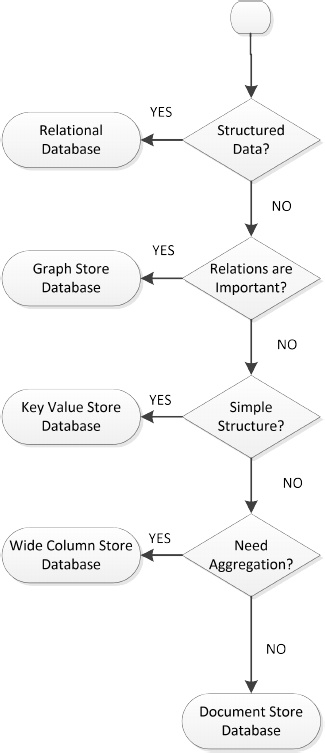
\includegraphics[width=8cm]{decision-flow.jpg}
			\centering
		\end{figure}
		\newpage
		\vfill

	\subsection{NoSQL Datenbanken}

		\begin{tabular} {| l | c | c | c | c | c | c |}
			\hline
			& Cassandra & HBase & MongoDB & Riak & MySQL Cluster & Couchbase		\\ \hline \hline
			Funktionalität &  &	 &  &  &  &  &		\\ \hline
			Zuverlässigkeit &  &	 &  &  &  &  &	 			\\ \hline
			Benutzbarkeit &  &	 &  &  &  &  &	 		\\ \hline
			Efizienz &  &	 &  &  &  &  &			\\ \hline
			Änderbarkeit &  &  &  &  &  &  &		\\ \hline 
			Übertragbarkeit	&  &	&  &  &  &  &					\\ \hline
		\end{tabular}

	\subsection{Rationale Datenbanken}
		
		\begin{tabular} {| l | c | c | c | c | c | c |}
			\hline
			& Sybase & IBM DB2 & Oracle & Microsoft SQL Server & MySQL & PostgreSQL	\\ \hline \hline
			Funktionalität &  &	 &  &  &  &  &		\\ \hline
			Zuverlässigkeit &  &	 &  &  &  &  &	 			\\ \hline
			Benutzbarkeit &  &	 &  &  &  &  &	 		\\ \hline
			Efizienz &  &	 &  &  &  &  &			\\ \hline
			Änderbarkeit &  &  &  &  &  &  &		\\ \hline 
			Übertragbarkeit	&  &	&  &  &  &  &					\\ \hline
		\end{tabular}

	\newpage
	\subsection{Data Mining \& Data Analysis}
	Durch die Sensoren im Auto sowie durch die zusätzlich durch den CarPC angebrachten wird eine enomre Menge an Daten geliefert. All diese Daten ergeben jedoch erst einen \"Sinn\", wenn wir sie mit geeigneten Verfahren analysieren und auswerten können. 

		\subsubsection{Frameworks}

		\begin{tabular} {| l | c | c | c | c | c | c |}
			\hline
			& RapidMiner & WEKA &  R-Programming & Orange & KNIME & NLTK		\\ \hline \hline
			Funktionalität &  &	 &  &  &  &  &		\\ \hline
			Zuverlässigkeit &  &	 &  &  &  &  &	 			\\ \hline
			Benutzbarkeit &  &	 &  &  &  &  &	 		\\ \hline
			Efizienz &  &	 &  &  &  &  &			\\ \hline
			Änderbarkeit &  &  &  &  &  &  &		\\ \hline 
			Übertragbarkeit	&  &	&  &  &  &  &					\\ \hline
		\end{tabular}

